\documentclass[border=3pt]{standalone}
% Preâmbulo compartilhado pelos diagramas TikZ da aula 9 de IHR (Robôs na Sociedade)
\usepackage[T1]{fontenc}
\usepackage[utf8]{inputenc}
\usepackage{lmodern}
\usepackage{amsmath}
\usepackage{xcolor}
\usepackage{tikz}
\usetikzlibrary{arrows.meta,angles,quotes,decorations.pathmorphing,decorations.pathreplacing,calc,
                positioning,shapes.geometric,shapes.misc,backgrounds,fit,
                math}

% Paleta (mesma dos SVGs originais)
% Paleta da disciplina de IHR: acento azul (#1A6FB5), cor de destaque do tema.
% (o nome "dblue" é mantido para não alterar todos os diagramas)
\definecolor{dblue}{HTML}{1A6FB5}
\definecolor{dorange}{HTML}{B3541E}
\definecolor{dgreen}{HTML}{4A7C59}
\definecolor{dred}{HTML}{9C4B4B}
\definecolor{dcream}{HTML}{F4F1EA}
\definecolor{dshade}{HTML}{DDD7C9}

% Função gaussiana (não normalizada por padrão de escala visual)
\pgfmathdeclarefunction{gauss}{3}{%
  \pgfmathparse{1/(#3*sqrt(2*pi))*exp(-((#1-#2)^2)/(2*#3^2))}%
}

% Estilos comuns (prefixo d... para não colidir com chaves internas do pgf)
\tikzset{
  >={Stealth[length=2mm]},
  dguide/.style={gray!55, dashed, line width=0.4pt},
  daxis/.style={gray!60, line width=0.7pt, ->},
  dbody/.style={fill=black!3, draw=black!80, line width=1pt},
  dacc/.style={draw=dblue, line width=1pt},
  dlbl/.style={black!55, font=\small},
  dsub/.style={black!45, font=\footnotesize},
  dstate/.style={circle, draw=black!80, fill=dcream, line width=1pt,
                 minimum size=17mm, font=\large, inner sep=1pt},
  dobs/.style={circle, draw=black!80, fill=dshade, line width=1pt,
               minimum size=14mm, font=\large, inner sep=1pt},
  dbox/.style={rounded corners=2pt, draw=black!80, fill=dcream, line width=1pt,
               align=center, inner sep=6pt},
  dop/.style={circle, draw=black!80, fill=white, line width=1pt,
              minimum size=6mm, inner sep=0pt, font=\small},
  dtrans/.style={->, dblue, line width=1pt},
  dmeas/.style={->, dorange, line width=1pt},
  dcurve/.style={line width=1pt, dblue},
  dcurveb/.style={line width=1.4pt, dorange},
}

\begin{document}
\hyphenpenalty=10000 \exhyphenpenalty=10000 \tolerance=9999 \emergencystretch=3em
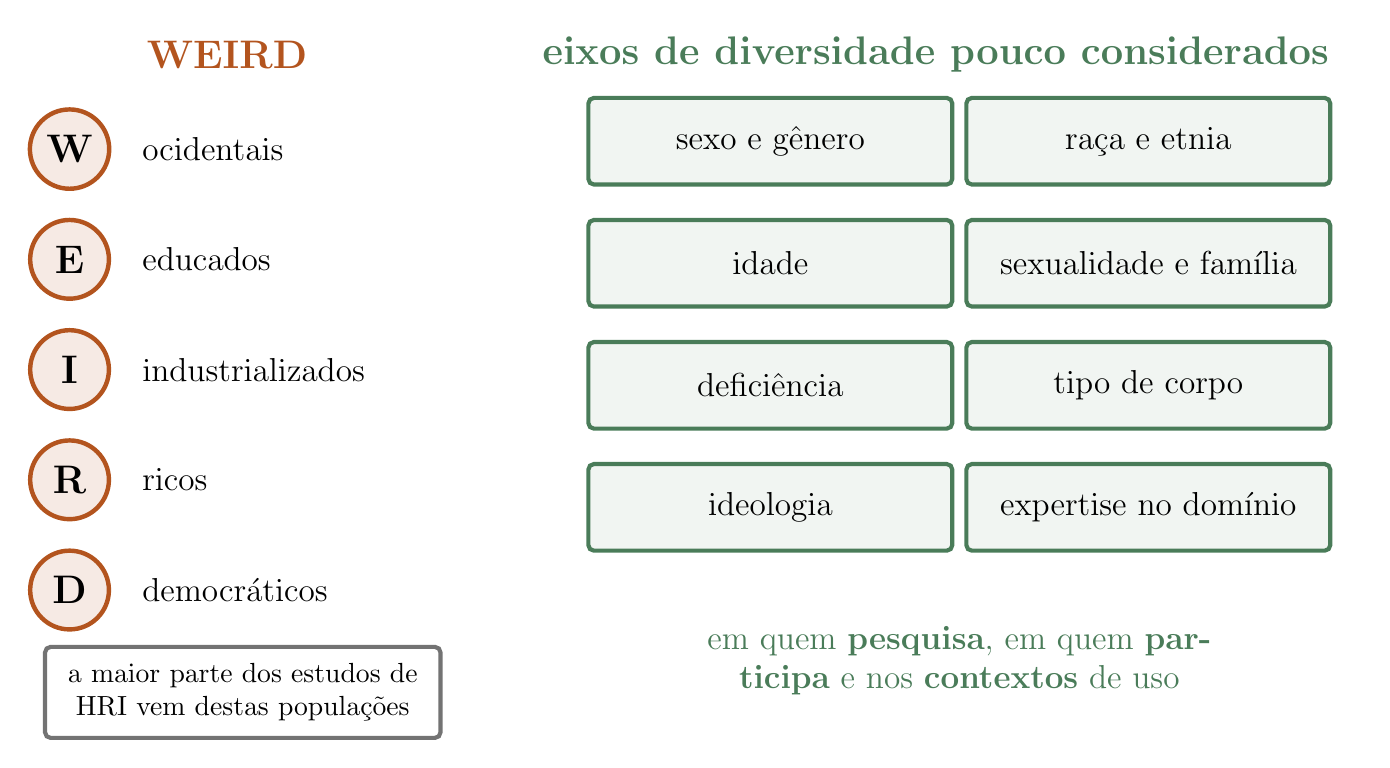
\begin{tikzpicture}[x=1cm,y=1cm]
\node[circle, draw=dorange, fill=dorange!12, line width=1.6pt, minimum size=1.0cm, font=\Large\bfseries] at (1.0,7.2) {W};
\node[font=\large, anchor=west] at (1.8,7.2) {ocidentais};
\node[circle, draw=dorange, fill=dorange!12, line width=1.6pt, minimum size=1.0cm, font=\Large\bfseries] at (1.0,5.800000000000001) {E};
\node[font=\large, anchor=west] at (1.8,5.800000000000001) {educados};
\node[circle, draw=dorange, fill=dorange!12, line width=1.6pt, minimum size=1.0cm, font=\Large\bfseries] at (1.0,4.4) {I};
\node[font=\large, anchor=west] at (1.8,4.4) {industrializados};
\node[circle, draw=dorange, fill=dorange!12, line width=1.6pt, minimum size=1.0cm, font=\Large\bfseries] at (1.0,3.000000000000001) {R};
\node[font=\large, anchor=west] at (1.8,3.000000000000001) {ricos};
\node[circle, draw=dorange, fill=dorange!12, line width=1.6pt, minimum size=1.0cm, font=\Large\bfseries] at (1.0,1.6000000000000005) {D};
\node[font=\large, anchor=west] at (1.8,1.6000000000000005) {democráticos};
\node[font=\Large\bfseries, dorange] at (3.0,8.4) {WEIRD};
\node[dbox, draw=black!55, fill=white, line width=1.5pt, text width=4.6cm, minimum height=1.1cm, font=\normalsize] at (3.2,0.3) {a maior parte dos estudos de HRI vem destas populações};
\node[font=\Large\bfseries, dgreen] at (12.0,8.4) {eixos de diversidade pouco considerados};
\node[dbox, draw=dgreen, fill=dgreen!8, line width=1.5pt, text width=4.2cm, minimum height=1.1cm, font=\large] at (9.9,7.3) {sexo e gênero};
\node[dbox, draw=dgreen, fill=dgreen!8, line width=1.5pt, text width=4.2cm, minimum height=1.1cm, font=\large] at (14.7,7.3) {raça e etnia};
\node[dbox, draw=dgreen, fill=dgreen!8, line width=1.5pt, text width=4.2cm, minimum height=1.1cm, font=\large] at (9.9,5.75) {idade};
\node[dbox, draw=dgreen, fill=dgreen!8, line width=1.5pt, text width=4.2cm, minimum height=1.1cm, font=\large] at (14.7,5.75) {sexualidade e família};
\node[dbox, draw=dgreen, fill=dgreen!8, line width=1.5pt, text width=4.2cm, minimum height=1.1cm, font=\large] at (9.9,4.199999999999999) {deficiência};
\node[dbox, draw=dgreen, fill=dgreen!8, line width=1.5pt, text width=4.2cm, minimum height=1.1cm, font=\large] at (14.7,4.199999999999999) {tipo de corpo};
\node[dbox, draw=dgreen, fill=dgreen!8, line width=1.5pt, text width=4.2cm, minimum height=1.1cm, font=\large] at (9.9,2.6499999999999995) {ideologia};
\node[dbox, draw=dgreen, fill=dgreen!8, line width=1.5pt, text width=4.2cm, minimum height=1.1cm, font=\large] at (14.7,2.6499999999999995) {expertise no domínio};
\node[font=\large, dgreen, text width=10cm, align=center] at (12.3,0.7) {em quem \textbf{pesquisa}, em quem \textbf{participa} e nos \textbf{contextos} de uso};
\end{tikzpicture}
\end{document}
